%% PREAMBLE
\documentclass[12pt, twoside]{report}

%% TODO: Add your useful packages here
\usepackage[utf8]{inputenc}
\usepackage[main=english,vietnamese]{babel}

\usepackage{amsmath}
\usepackage{amssymb}

%% TODO: Use \cmark for tick and \xmark for x
\usepackage{pifont}
\newcommand{\cmark}{\ding{51}}%
\newcommand{\xmark}{\ding{55}}%

\usepackage{multirow}
\usepackage{graphicx}
\usepackage{tikz}
\usetikzlibrary{calc}

\usepackage[a4paper, top=2.5cm, bottom=2cm, left=3cm, right=2cm, bindingoffset=5mm]{geometry}
\usepackage{fancyhdr}
\usepackage{titlesec}

\usepackage{algorithm}
\usepackage{algpseudocode}
\usepackage{url}
\usepackage{listings}
\usepackage{xcolor}

%% Customize JavaScript listings, Python do not need this
\lstdefinestyle{mystyle}{
	basicstyle=\ttfamily\footnotesize,
	breakatwhitespace=false,
	breaklines=true,
	captionpos=b,
	frame=single,
	keepspaces=true,
	numbers=left,
	numbersep=5pt, 
	numberstyle=\tiny\color{black},
	showstringspaces=false,
}

\lstset{style=mystyle}
\lstdefinelanguage{JavaScript}{
	morekeywords=[1]{break, continue, delete, else, for, function, if, in,
	new, return, this, typeof, var, void, while, with},
	morekeywords=[2]{false, null, true, boolean, number, undefined,
	Array, Boolean, Date, Math, Number, String, Object},
	morekeywords=[3]{eval, parseInt, parseFloat, escape, unescape},
	sensitive,
	morekeywords=[4]{await, async, case, catch, class, const, default, do,
		enum, export, extends, finally, from, implements, import, instanceof,
	let, static, super, switch, throw, try},
	morecomment=[s]{/*}{*/},
	morecomment=[l]//,
	morecomment=[s]{/**}{*/},
	morestring=[b]',
	morestring=[b]",
	keywordstyle={[1]\color{teal}\bfseries},
	keywordstyle={[2]\color{red}\bfseries},
	keywordstyle={[3]\color{violet}\bfseries},
	keywordstyle={[4]\color{blue}\bfseries},
	commentstyle=\color{gray}\ttfamily,
	stringstyle=\color{orange}\ttfamily,
}

%% Customize chapter titles
\titleformat{\chapter}[display]
  {\Huge\bfseries\centering}{\chaptername~\thechapter}
  {0pt}                        
  {\Huge}                     
\titlespacing*{\chapter}
  {0pt}                   
  {*0}                          
  {1em}
                     
%% Fix appendix labeling
\makeatletter
\newcommand\AppendixName{Appendix}
\let\oldappendix\appendix
\renewcommand{\appendix}{%
  \oldappendix
  \renewcommand{\chaptername}{\AppendixName}  \renewcommand{\thechapter}{\@Alph\c@chapter}}
\makeatother
\addto\captionsenglish{\renewcommand*\contentsname{Table of Contents}}
\addto{\extrasenglish}{%
  \renewcommand{\bibname}{References}
}
\renewcommand\lstlistlistingname{List of Listings}

%% TODO: Put all the figure files inside the images folder
\graphicspath{{images/}}

\begin{document}
\pagenumbering{roman}

\newgeometry{top=2.5cm, bottom=2.5cm, left=2.5cm, right=2.5cm}

%% TODO: Add information to the Title page
\begin{titlepage}

	\begin{tikzpicture}[remember picture,overlay,inner sep=0,outer sep=0]
     \draw[blue!70!black,line width=4pt] ([xshift=-1.5cm,yshift=-2cm]current page.north east) coordinate (A)--([xshift=1.5cm,yshift=-2cm]current page.north west) coordinate(B)--([xshift=1.5cm,yshift=2cm]current page.south west) coordinate (C)--([xshift=-1.5cm,yshift=2cm]current page.south east) coordinate(D)--cycle;

     \draw ([yshift=0.5cm,xshift=-0.5cm]A)-- ([yshift=0.5cm,xshift=0.5cm]B)--
     ([yshift=-0.5cm,xshift=0.5cm]B) --([yshift=-0.5cm,xshift=-0.5cm]B)--([yshift=0.5cm,xshift=-0.5cm]C)--([yshift=0.5cm,xshift=0.5cm]C)--([yshift=-0.5cm,xshift=0.5cm]C)-- ([yshift=-0.5cm,xshift=-0.5cm]D)--([yshift=0.5cm,xshift=-0.5cm]D)--([yshift=0.5cm,xshift=0.5cm]D)--([yshift=-0.5cm,xshift=0.5cm]A)--([yshift=-0.5cm,xshift=-0.5cm]A)--([yshift=0.5cm,xshift=-0.5cm]A);


     \draw ([yshift=-0.3cm,xshift=0.3cm]A)-- ([yshift=-0.3cm,xshift=-0.3cm]B)--
     ([yshift=0.3cm,xshift=-0.3cm]B) --([yshift=0.3cm,xshift=0.3cm]B)--([yshift=-0.3cm,xshift=0.3cm]C)--([yshift=-0.3cm,xshift=-0.3cm]C)--([yshift=0.3cm,xshift=-0.3cm]C)-- ([yshift=0.3cm,xshift=0.3cm]D)--([yshift=-0.3cm,xshift=0.3cm]D)--([yshift=-0.3cm,xshift=-0.3cm]D)--([yshift=0.3cm,xshift=-0.3cm]A)--([yshift=0.3cm,xshift=0.3cm]A)--([yshift=-0.3cm,xshift=0.3cm]A);

   \end{tikzpicture}

   
	\centering
	\textbf{VIETNAM NATIONAL UNIVERSITY OF HO CHI MINH CITY}\par \textbf{THE
		INTERNATIONAL UNIVERSITY}\par \textbf{SCHOOL OF COMPUTER SCIENCE AND ENGINEERING}\par
														
	\vspace{1.5cm}
	
\includegraphics[width=0.3\textwidth]{IU.png}
														
	\vspace{1.5cm}
\textbf{\large Implementing a Test Generation Service \\ For Flutter Framework}
														
	\vspace{1.5cm}
	By \par \textbf{Dao Minh Huy}
														
	\vspace{4.5cm}
	\textit{A thesis submitted to the School of Computer Science and Engineering \\ 
    in partial fulfillment of the requirements for the degree of \\ Bachelor of Computer Science}
														
	\vspace{3.5cm}
	\text{Ho Chi Minh City, Vietnam} \par June 2025
														
	\newpage
													
	%% TODO: Add committee names to the Signature page
	\centering
														
	\textbf{\large Implementing a Test Generation Service \\ For Flutter Framework}\par
	\vspace{4cm}
														
	\hspace{7cm}
	\makebox[7cm][l]{\text{APPROVED BY:}}
	\par
	\vspace{2cm}
														
	\hspace{7cm}
	\makebox[7cm][l]{\underline{\hspace{7cm}}}
	\par \hspace{7cm}
	\makebox[7cm][l]{\textit{Committee name here}}
	\par
	\vspace{2cm}
														
	\hspace{7cm}
	\makebox[7cm][l]{\underline{\hspace{7cm}}}
	\par \hspace{7cm}
	\makebox[7cm][l]{\textit{Committee name here}}
	\par
	\vspace{2cm}
														
	\hspace{7cm}
	\makebox[7cm][l]{\underline{\hspace{7cm}}}
	\par \hspace{7cm}
	\makebox[7cm][l]{\textit{Committee name here}}
	\par
	\vspace{2cm}
														
	\hspace{7cm}
	\makebox[7cm][l]{\underline{\hspace{7cm}}}
	\par \hspace{7cm}
	\makebox[7cm][l]{\textit{Committee name here}}
	\par
	\vspace{2cm}
			
	\hspace{7cm}
	\makebox[7cm][l]{\underline{\hspace{7cm}}}
	\par \hspace{7cm}
	\makebox[7cm][l]{\textit{Committee name here}}
	\par
	\vspace{0.75cm}
														
	\hspace{7cm}
	\makebox[7cm][r]{\text{THESIS COMMITTEE}}
	\par
	\thispagestyle{empty}
\end{titlepage}
\restoregeometry
	
%% TODO: Acknowledgments page
\chapter*{Acknowledgments}
\hspace{1cm}It is with profound gratitude and sincere appreciation that I extend my heartfelt thanks to Dr. Tran Thanh Tung for his unwavering support and exceptional professional guidance throughout the course of this thesis. His dedication, insightful feedback, and encouragement provided me with the optimal conditions to carry out and complete this research successfully. Dr. Tran Thanh Tung's invaluable knowledge and expertise have been a constant source of motivation and inspiration, significantly contributing to my learning process and academic growth.

\hspace{0.5cm}I also want to express my thanks to all professors and lecturers who have followed and instructed me throughout my university journey. Their expertise and experience have enlightened and sharpened my skills to confidently enter the industry.

\hspace{0.5cm}Lastly, I sincerely thank the thesis evaluation committee for their valuable time reviewing and assessing this thesis.

\thispagestyle{empty}

%% Add Table of Contents, List of Figures, List of Tables pages
\tableofcontents
\listoftables
\addcontentsline{toc}{chapter}{List of Tables}
\listoffigures
\addcontentsline{toc}{chapter}{List of Figures}
\listofalgorithms
\addcontentsline{toc}{chapter}{List of Algorithms}
\lstlistoflistings
\addcontentsline{toc}{chapter}{List of Listings}

%% TODO: Abstract page (iv, printed)
\chapter*{Abstract}
\addcontentsline{toc}{chapter}{Abstract}
Software testing is indispensable for ensuring the reliability and correctness of any software product before deployment. Despite its importance, developers often find writing unit tests and integration tests tedious and time-consuming. This is not due to the complexity of the process but to the cognitive effort required to work retrospectively, evaluating and validating code logic that has already been implemented without being bias from the logic of the source code. \\
This thesis introduces an innovative approach leveraging the capabilities of Artificial Intelligence (AI) called “Test Genie”, which will alleviate developers' workloads by automating the generation of test cases. By offloading the task of test generation to an AI-driven system, developers can concentrate entirely on writing robust and functional source code. The proposed solution employs the Retrieval-Augmented Generation (RAG) technique to enhance the quality and relevance of the generated test cases, ensuring that the results align with the intended behavior of the code. \\
To further validate the practicality of the system, the service incorporates an embedded Software Development Kit (SDK) for the supported platform, with the initial implementation focused on the Flutter framework. This integration ensures that the AI-generated test files adhere to the platform's standards and are executable without manual intervention. \\
The results of this research aim to demonstrate how AI can transform the software testing process, reducing developer effort, improving testing efficiency, and fostering higher-quality code in modern software development.


%% TODO: Add \chapter{Chapter name} followed by \input{chapters/filename} if you need more chapter or modify them
\chapter{INTRODUCTION}
\pagenumbering{arabic}
\setcounter{page}{1}
%% TODO: Make sure to use \textbf or \textit for highlighting keywords, and \cite{} to cite the corresponding quotations
\section{Background}
As software systems become increasingly complex, the demand for rigorous software testing has grown significantly. Modern applications often integrate multiple components, rely on distributed architectures, and interact with various external systems, making them more vulnerable to errors. According to a study by Capgemini (2021), the average cost of software failures has risen by 15\% annually~\cite{WQR2122}, underscoring the need for comprehensive testing to ensure reliability. Furthermore, the adoption of agile and DevOps methodologies has accelerated development cycles, necessitating continuous testing to maintain quality. The World Quality Report (2022) highlights that 78\% of organizations have increased their investment in testing tools and resources over the past five years~\cite{WQR2122}, reflecting the growing recognition of testing as a critical component of software development. Due to high demand in software testing, the market value of digital assurance also get higher. The average annual salary of Quality assurance tester have increased, from 60,000\$ in 2015 to 82,000\$ in 2024~\cite{QASalaries}.

\section{Problem Statement}

\hspace{0.5cm} The rapid evolution of technology has led to the proliferation of programming languages and development frameworks, each with unique features and ecosystems. While this diversity offers developers powerful tools and improved syntax to enhance productivity, it also introduces significant challenges in the testing process. Developers must familiarize themselves with different testing languages, frameworks, and techniques for each platform, which can be both time-consuming and error-prone.

\hspace{0.2cm} Although languages and frameworks are getting better in both syntax and community support, the testing process also getting trickier. Writing comprehensive unit and integration tests often requires developers to think “backtrackingly,” reconstructing potential use cases and edge cases after implementing the functionality. A human can overlooking critical edge cases that might cause a costly consequence. According to CISQ, poor software cost the U.S. economy \$2.08 trillion in 2020 alone~\cite{CostPoorSoftware}.

\hspace{0.2cm} To address these challenges, this thesis proposes the integration of an AI-driven Test Generation Service named Test Genie. By leveraging Large Language Models (LLMs), this service automates the creation of test cases, significantly reducing the burden on developers. Automating this process not only optimizes resource allocation but also minimizes the potential for human error, ensuring a more thorough and systematic approach to software testing.


\section{Scope and Objectives}

\hspace{0.2cm}Initially, this thesis will only focus on one single framework: Flutter - a cross-platfrom framework that can build the product for many platform from one source code. Although Flutter is considered a new framework but the support community and the usage of this framework is increasing every year. This framework also support a testing module, enable users to develop different testing packages and techniques. The research will assess the feasibility of AI in test cases generation by using Langchain library to integrate API of LLM models. By using multiple LLM models, the thesis aim to present a suitable methodology that could provide support to reduce QA testers and developers's workload and effectively cover edge cases that human often miss.

\hspace{0.2cm}To successfully implement this service, three primary objectives must be achieved. First, the AI must demonstrate the capability to analyze the business model and functional requirements directly from the project source code. This requires understanding the logical structure and intent of the application. Second, the AI must leverage an effective test generator model capable of producing test cases that align with the platform's standards while maintaining relevance to the identified business logic. Third, the generated code must be thoroughly validated to ensure its correctness and compatibility within the Flutter ecosystem. By meeting these requirements, the proposed service aims to establish a reliable and efficient solution for automating test case generation.

%% TODO: Use enumerate environment to start an ordered list, while using itemize environment to start an unordered list
% \begin{enumerate}
% 	\item This is the first \textbf{bold keyword} of the ordered list to emphasize an important concept.
% 	\item The second point in the ordered list addresses \textbf{another key idea} in the discussion.
% 	      \begin{itemize} 	
% 	      	\item This is the first \textbf{bold keyword} of the unordered list to emphasize an important concept.
% 	      	\item The second point addresses \textit{italic keyword} in the unordered list discussion.
% 	      \end{itemize}
% \end{enumerate}

\hspace{0.2cm}In this thesis, we will work on three components:
\begin{itemize}
	\item[-] Business Logic Analyzer module (BLA)
	\item[-] AI-integrated test generation module
	\item[-] AI test validation module
\end{itemize}
\hspace{0.2cm}Each component will share the same tech stack:
\begin{itemize}
	\item[-] Python~\cite{PyMachineLearning}: This is a popular high-level language that used widely by AI developers. Its simple syntax and wide range of supportive library help developers effectively implement complex system with minimal syntax.
	\item[-] Python-Flask~\cite{flask}: This is a micro web framework for Python. It is lightweight and easy to use, making it suitable for building small to medium-sized web applications. 
	\item[-] Python-Langchain~\cite{langchain}: Langchain is a framework for developing applications powered by Large Language Models (LLMs). This is an open-source framework and effectively utilize API provided by LLMs service provider as well as self-hosted LLMs.
\end{itemize}

\section{Structure of thesis}
This thesis consist of six chapters:
\begin{itemize}
	\item[-] \textbf{Chapter 1. Introduction:} Introduce the background story, how I identify the problem as well as the scope and objectives of this research. This chapter also lightly introduce the proposed solution of the stated problem.
	\item[-] \textbf{Chapter 2. Liturature review/Related work:} This chapter focus on the related work that contributed to the thesis.
	\item[-] \textbf{Chapter 3. Methodology:} Presenting the methodology behind the project, including the component of the system, method implemented for each module and the plan to validate the generated test from AI.
	\item[-] \textbf{Chapter 4. Implement and results:} This chapter summarize the design and implementations of the system as well as the result of this research.
	\item[-] \textbf{Chapter 5. Discussion and evaluation:} In this chapter, we will evaluate the result of this system.
	\item[-] \textbf{Chapter 6. Conclusion and future work:} This chapter will conclude the research of this thesis, as well as the plan of development in the future. 
\end{itemize}

\chapter{RELATED WORK}
%% TODO: Make sure to use \textbf or \textit for highlighting keywords, and \cite{} to cite the corresponding quotations

% TODO: Fake references, pls rewrite this base on this outline
\section{Unit test generator}

\paragraph{Evolution of Test Generation Approaches.} Software testing has evolved significantly over the decades, transitioning from purely manual testing to increasingly automated approaches. The earliest automated test generation methods emerged in the 1970s with simple input-output validation techniques~\cite{TestHistory}. By the 1990s, more sophisticated approaches began to appear, including symbolic execution and model-based testing. The 2000s saw the rise of search-based software testing (SBST), which applies metaheuristic search techniques to generate test cases that satisfy specific coverage criteria~\cite{SearchBasedSurvey}. In parallel, constraint-based testing evolved to leverage constraint solvers for generating test inputs that exercise specific code paths. Random testing, despite its simplicity, has remained relevant due to its ability to discover unexpected failures with minimal assumptions about the system under test.

\hspace{0.5cm} These traditional approaches have dominated the automated testing landscape until recently, when the emergence of advanced artificial intelligence techniques, particularly Large Language Models (LLMs), introduced a paradigm shift in how test generation can be approached. Unlike previous methods that relied on explicit algorithms or search strategies, LLM-based approaches leverage patterns learned from vast corpora of code to generate tests that more closely resemble those written by human developers.

\paragraph{LLMs approach compared to formulated approach.} To accurately give test case with correct syntax, I have researched some techniques that can handle different frameworks with just one centrialized system. There is a research that compares the performance of some common approaches including search-based, constraint-based and random-based. Tests generated by these methods frequently lack meaningful structure or descriptive naming conventions, making them difficult for developers to interpret and modify ~\cite{UnitTest}. This limitation can hinder their practical usability, particularly in dynamic and iterative development environments.

\hspace{0.5cm} In contrast, test case generation using Large Language Models (LLMs) offers a more intuitive and human-aligned approach~\cite{UnitTest}. LLMs, trained on vast amounts of programming-related data, possess the capability to generate test cases that not only adhere to syntactical correctness but also align closely with human developers' intentions and coding practices. This alignment results in unit tests that are more readable, contextually relevant, and easier to understand. Developers can quickly adjust and refine these tests as needed, enhancing their utility in real-world scenarios.

\hspace{0.5cm} Moreover, the flexibility of LLMs enables them to adapt seamlessly to various programming languages and frameworks, providing a centralized solution for diverse development ecosystems. While traditional approaches may produce marginally higher percentages of technically correct test cases, they often lack the usability and adaptability that LLM-based methods provide. As a result, services leveraging LLMs for test generation consistently receive more favorable user feedback due to their focus on developer experience, ease of use, and alignment with real-world development workflows.

\paragraph{Quantitative Analysis of Test Generation Approaches.} Recent empirical studies have provided quantitative evidence comparing traditional and LLM-based test generation approaches across multiple dimensions. According to a comprehensive benchmark study by Gabriel et al.~\cite{TestBenchmark}, test cases generated by LLMs achieved an average of 76\% code coverage compared to 82\% from specialized constraint-based tools. However, when measuring test suite maintainability using the Test Maintainability Index (TMI), LLM-generated tests scored significantly higher with an average score of 68 compared to 42 for traditional methods. This highlights a fundamental trade-off between technical perfection and practical usability.

\hspace{0.5cm} Table~\ref{tab:test-gen-comparison} provides a comparative analysis of different test generation approaches based on several key metrics, synthesized from multiple research studies~\cite{UnitTest, TestBenchmark, LLMTestComparison}.

\begin{table}[ht]
	\centering
	\caption{Comparison of Test Generation Approaches}
	\label{tab:test-gen-comparison}
	\resizebox{\textwidth}{!}{%
		\begin{tabular}{lcccc}
			\hline
			\textbf{Metric} & \textbf{Search-based} & \textbf{Constraint-based} & \textbf{Random-based} & \textbf{LLM-based} \\ \hline
			Code Coverage & High (75-85\%) & Very High (80-90\%) & Medium (50-65\%) & High (70-80\%) \\
			Test Readability & Low & Medium & Very Low & Very High \\
			Naming Conventions & Poor & Moderate & Poor & Good to Excellent \\
			Framework Adaptability & Low & Low & Medium & High \\
			Edge Case Detection & Medium & High & Medium-High & Medium \\
			Maintenance Effort & High & Medium & High & Low \\
			Generation Speed & Fast & Slow & Very Fast & Medium \\
			Developer Satisfaction & Low & Medium & Low & High \\
			\hline
		\end{tabular}%
	}
\end{table}

\hspace{0.5cm} The data reveals that while traditional methods may excel in specific technical metrics like edge case detection (particularly constraint-based approaches), LLM-based methods offer a more balanced profile with particular strengths in human-centric metrics such as readability and maintainability. This balance makes LLM-based approaches especially suitable for industrial applications where developer productivity and code maintainability are primary concerns.

\paragraph{Disadvantages of  LLMs.}One of the most significant challenges is their propensity to generate hallucinations, where the model produces incorrect or fabricated outputs that lack grounding in factual data. This issue is particularly critical in tasks requiring precision, such as author attribution. For instance, research introducing the Simple Hallucination Index (SHI) revealed that even advanced LLMs like Mixtral 8x7B, LLaMA-2-13B, and Gemma-7B suffered from hallucinations, with Mixtral 8x7B achieving an SHI as high as 0.87 for certain datasets ~\cite{LLMLimitations}. These hallucinations undermine the reliability and trustworthiness of LLMs, especially in contexts where factual accuracy is crucial. 

\hspace{0.5cm} Another drawback of LLMs is their lack of transparency in decision-making. These models function as black boxes, providing little insight into the reasoning behind their outputs ~\cite{LLMLimitations}. This opacity complicates the debugging process and limits the ability to verify results, which is particularly problematic in applications requiring a high degree of explainability. Additionally, LLMs are highly dependent on the quality and diversity of their training data. Biases or inaccuracies present in the data can result in outputs that reinforce those biases or produce flawed results. Moreover, while these models excel at generating output based on their training corpus, they often struggle to generalize effectively when faced with novel or unseen cases.

\paragraph{LLM Limitations in Testing Contexts.} While general LLM limitations are well-documented, their specific impact on test generation presents unique challenges. Test generation requires a deep understanding of program semantics, expected behaviors, and framework-specific testing conventions. Wang et al.~\cite{LLMTestingLimitations} identified several testing-specific limitations in their comprehensive evaluation of LLM-based testing tools:

\hspace{0.5cm} First, LLMs frequently generate \textbf{syntactically valid but semantically incorrect} tests, particularly when dealing with complex object relationships or state-dependent behaviors. In their study, approximately 32\% of generated tests contained semantic errors despite being syntactically correct. Second, LLMs demonstrate \textbf{inconsistent mocking behavior}, struggling to correctly identify which components should be mocked in unit tests and how to implement those mocks appropriately. Third, there exists a \textbf{framework understanding gap}, where LLMs may mix testing conventions from different frameworks or misapply testing patterns.

\hspace{0.5cm} These limitations highlight the need for specialized approaches when applying LLMs to test generation tasks. Solutions proposed in recent literature include fine-tuning models on framework-specific testing examples, implementing post-processing validation steps, and incorporating human feedback loops to refine and correct generated tests~\cite{LLMTestEnhancements}.

\section{Understanding Business Logic}

\paragraph{The concept of Business Logic.} An industry's business logic can be seen as a description of a number of basic conditions or circumstances that make up important starting points for understanding an established business and its conditions for change~\cite{BusinessRules}. It encodes the real-world policies, procedures, and processes that govern how data is created, managed, and manipulated in a way that aligns with the objectives of the organization. Business logic acts as the foundation for decision-making and operational tasks, ensuring that the software performs actions that mirror the intended business behavior. This could involve calculating prices, validating transactions, or managing inventory, all based on predefined rules and conditions derived from the organization's requirements.

\hspace{0.5cm}Business logic serves as the intellectual layer of an application, translating business needs into functional processes that can be executed by the software. It defines the constraints, relationships, and actions that underpin the flow of data within the system, ensuring that each operation adheres to the intended policies and delivers accurate results. The clarity and accuracy of business logic are essential for maintaining the reliability of software systems, as it directly influences how well the software aligns with the real-world scenarios it is designed to address. By formalizing business rules into structured logic, it enables organizations to automate and scale their operations effectively while minimizing the risk of errors and inconsistencies.

\paragraph{Taxonomies of Business Rules.} Business rules can be categorized into several distinct types, each serving different purposes in the overall business logic architecture. Researchers have proposed various taxonomies to classify these rules. One widely accepted classification by von Halle~\cite{BusinessRulesTaxonomy} divides business rules into five primary categories:

\hspace{0.5cm} \textbf{Definitions} form the foundational terms and concepts within a business domain, establishing a common vocabulary. \textbf{Facts} express relationships between definitions, capturing the static structure of business information. \textbf{Constraints} represent business rules that restrict actions or states, enforcing boundaries on operations. \textbf{Derivations} are rules that calculate values or derive new facts from existing data, often implementing business formulas or algorithms. \textbf{Action enablers} trigger specific actions when certain conditions are met, representing the dynamic behavior of the system.

\hspace{0.5cm} Morgan~\cite{MorganBusinessRules} offers an alternative categorization focusing on implementation aspects: \textbf{Computational rules} perform calculations following specific algorithms; \textbf{Constraint rules} validate data against defined conditions; \textbf{Inference rules} draw conclusions based on existing facts; \textbf{Process control rules} govern workflow sequences. Understanding these taxonomies is crucial for effective extraction and representation of business logic in test generation systems, as different rule types require different testing approaches and validation strategies.

\paragraph{Existing method.} The extraction of business logic from source code has been a long-standing challenge, especially in the context of legacy systems. Traditionally, reverse engineering techniques have been employed to bridge the gap between low-level implementation details and high-level conceptual models of software systems. Tools such as SOFT-REDOC have been developed to support this process, particularly for legacy COBOL programs~\cite{BusinessRules}. These tools rely on program stripping, wherein non-essential code is eliminated to focus on the logic that directly affects specific business outcomes. This involves identifying critical variables and their assignments, conditions, and dependencies to reconstruct the underlying business rules.

\paragraph{Evolution of Business Logic Extraction.} Business logic extraction techniques have evolved considerably over time, adapting to changing programming paradigms and technologies. The earliest methods focused on manual code review and documentation, requiring domain experts to manually analyze source code and extract business rules~\cite{ManualBLExtraction}. This approach, while thorough, proved time-consuming and inconsistent. The 1990s saw the emergence of the first automated tools for COBOL and other legacy languages, primarily utilizing static analysis techniques to identify data manipulation patterns~\cite{BusinessRules}.

\hspace{0.5cm} Recent advances incorporate machine learning and natural language processing techniques. Hamdard and Lodin~\cite{MLBusinessLogic} demonstrated that supervised learning models could identify business logic components with 78\% accuracy after training on labeled code samples. Their approach particularly excelled at distinguishing between technical infrastructure code and actual business logic.

\paragraph{Challenges with Existing Approaches.} The reliance on human analysts to interpret outputs and dependencies makes the process time-consuming and error-prone~\cite{BusinessRules}. Furthermore, legacy programs often involve convoluted logic and scattered assignments, making it difficult to reconstruct business rules with precision. In cases where variable names and data structures lack descriptive clarity, analysts may struggle to comprehend the program's intent, leading to incomplete or inaccurate extraction of business logic. These limitations highlight the need for more automated and scalable approaches to understanding business logic in modern and legacy systems.

\section{Test Quality Assessment}

\paragraph{Metrics for Test Quality Evaluation.} Evaluating the quality of generated test cases is essential for determining their effectiveness and practical utility. Traditional test quality metrics focus primarily on coverage measurements, with code coverage being the most widely used. However, research by Inozemtseva and Holmes~\cite{TestCoverageLimitations} demonstrated that high coverage does not necessarily correlate with test effectiveness in detecting faults. This finding has prompted researchers and practitioners to develop more comprehensive quality metrics that consider multiple dimensions of test effectiveness.

\hspace{0.5cm} \textbf{Coverage metrics} remain valuable but insufficient indicators of test quality. Line coverage, branch coverage, and path coverage provide increasingly detailed insights into which portions of code are exercised by tests, with path coverage offering the most thorough assessment at the cost of computational complexity. \textbf{Mutation testing} represents a more robust approach to evaluating test effectiveness by introducing artificial faults (mutations) into the code and measuring how many mutations are detected by the test suite~\cite{MutationTesting}. A high mutation score indicates tests that are sensitive to changes in program behavior, suggesting better fault detection capability.

\hspace{0.5cm} Beyond technical effectiveness, \textbf{maintainability metrics} evaluate how easily tests can be understood and modified. Metrics such as cyclomatic complexity, test size, assertion density, and comment ratio contribute to an overall test maintainability index~\cite{TestMaintainability}. Studies by Bavota et al.~\cite{TestReadability} found that more maintainable tests are 42\% more likely to be regularly updated when the code they test changes, highlighting the practical importance of these metrics.

\paragraph{Comparing Generated Tests to Human-Written Tests.} % TODO: finish this shiet

\hspace{0.5cm} The gap between human and AI test generation has narrowed significantly with recent LLM-based approaches. In a follow-up study using more advanced LLMs, Gabriel et al.~\cite{TestBenchmark} found that professional developers could correctly identify the origin of tests (human vs. AI) only 58\% of the time, barely better than random chance. This suggests that modern AI approaches are producing tests increasingly indistinguishable from human-written ones in terms of style and structure, though gaps in domain understanding persist.

\section{Framework-Specific Testing Challenges}

\paragraph{Flutter Testing Ecosystem.} The Flutter framework presents unique testing challenges and opportunities due to its cross-platform nature and widget-based architecture. Flutter's testing ecosystem encompasses three primary testing levels: unit testing for individual functions and classes, widget testing for UI components, and integration testing for end-to-end application behavior~\cite{FlutterTesting}. Each level requires different testing approaches and introduces distinct challenges for automated test generation.

\hspace{0.5cm} Unit testing in Flutter follows standard Dart testing conventions but includes additional complexities when testing code that interacts with Flutter's widget system or platform channels. According to Pfaffen and Wannier.~\cite{FlutterTesting}, the most common challenge in Flutter unit testing is properly mocking dependencies, particularly those that interact with the Flutter framework or platform-specific code. Their analysis of open-source Flutter projects found that 64\% of unit test failures were related to improper mocking or dependency isolation.

\hspace{0.5cm} Widget testing represents a middle ground between unit and integration testing, focusing on testing UI components in isolation. Flutter's widget testing framework provides tools for rendering widgets, simulating user interactions, and verifying expected UI behavior. However, Pfaffen~\cite{FlutterTesting} also identified several challenges specific to widget testing, including handling asynchronous UI updates, managing widget lifecycles, and testing complex widget hierarchies. Their study found that widget tests written by novice Flutter developers had a 47\% higher failure rate than those written by experienced developers, highlighting the steep learning curve associated with effective widget testing.

\paragraph{Cross-Platform Testing Considerations.} Flutter's promise of a single codebase for multiple platforms introduces additional testing considerations. While the core application logic may be shared, platform-specific behaviors, interactions, and appearances often require targeted testing approaches. Research by Lukas Dagne~\cite{CrossPlatformTesting} found that 38\% of Flutter application bugs were platform-specific despite the shared codebase, with iOS-specific issues being 1.6 times more common than Android-specific issues in the studied applications.

\hspace{0.5cm} These framework-specific challenges highlight the need for specialized approaches when generating tests for Flutter applications. Effective test generation must account for Flutter's unique widget lifecycle, asynchronous programming model, and cross-platform considerations to produce meaningful and reliable tests.

%% TODO: Make sure to use \subsection{} and \subsubsection{} for smaller sections inside a larger sections
% \section{Theoretical Background}
% %% TODO: Use ~\ref{} to mention a labeled figure, table, section, or anything else
% \subsection{Concept 1}
% Sed eget lobortis leo. Maecenas ut tempor nibh. Nullam arcu nulla, aliquet vel enim maximus, gravida porta tortor. Orci varius natoque penatibus et magnis dis parturient montes, nascetur ridiculus mus. Donec aliquet luctus porttitor. Vivamus porta nulla ut tortor condimentum, at ullamcorper orci facilisis. Vivamus venenatis tellus vel dolor vestibulum, ac placerat orci laoreet. Praesent at elit arcu. Maecenas et lacus sit amet odio finibus semper. Mauris commodo vestibulum aliquam. Mauris non faucibus augue. Vivamus eleifend mauris eget mi venenatis, a maximus dolor mollis in Fig.~\ref{fig:1}.

% %% TODO: Adjust the size of the figure by using [widht=.x\linewidth] (x is a fraction) to fit within the page width. Then rename to your picture file name, add the caption and a label
% \begin{figure}[ht]
% 	\centering
% 	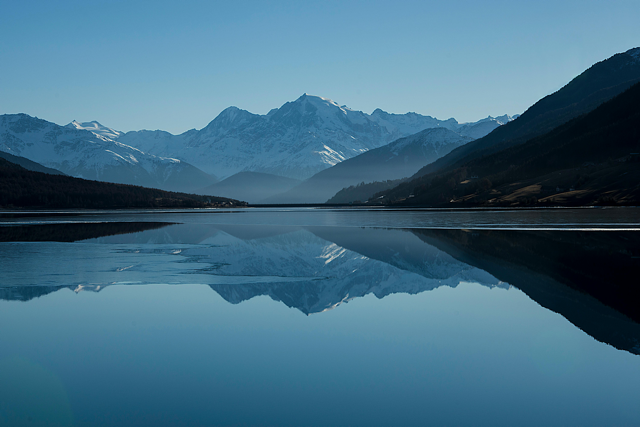
\includegraphics[width=\linewidth]{sample.png}
% 	\caption{The caption of the figure.}
% 	\label{fig:1}
% \end{figure}

% \subsubsection{More details of Concept 1}
% Quisque sit amet ipsum sed ligula congue mattis viverra sit amet sem. Phasellus ante tortor, dictum id ex eget, lacinia pulvinar ligula. Aenean sodales in augue in tempus. Ut ut venenatis magna, feugiat tristique justo. Etiam ac mauris cursus, tincidunt elit commodo, molestie dolor. Nam maximus feugiat nunc, et facilisis eros malesuada vel. Suspendisse potenti. Cras ipsum eros, cursus vitae luctus ac, blandit pulvinar velit. Donec cursus viverra aliquet. Maecenas pharetra nec sem a gravida provided in Table~\ref{tab:1}.

% \begin{table}[ht]
% 	\centering
% 	\caption{Comparison of different methods (\protect\cmark: YES, \protect\xmark: NO).}
% 	\label{tab:1}
% 	%% Comment the next line if the table width is relatively small
% 	\resizebox{\textwidth}{!}{%
% 		\begin{tabular}{lcccccc}
% 			\hline
% 			          & \textbf{Your Method} & Method B & Method C & Method D & Method E & Method F \\ \hline
% 			Feature 1 & \cmark               & \cmark   & \xmark   & \cmark   & \xmark   & \cmark   \\ 
% 			Feature 2 & \cmark               & \xmark   & \cmark   & \cmark   & \cmark   & \xmark   \\ 
% 			Feature 3 & \xmark               & \cmark   & \cmark   & \xmark   & \xmark   & \cmark   \\ 
% 		\end{tabular}%
% 		%%TODO: Also comment this } to match the above command
% 	}
% \end{table}
	
	
% %% TODO: For math mode, wrap the equation inside $ $ for inline mode, wrap inside $$ $$ for non-numbering block mode, or align environment as a numbered block equation
% Ut consectetur quam in elit ullamcorper, non dictum velit congue. Nulla facilisi. Suspendisse potenti. Donec ut felis nec odio tempor rhoncus non a ex $\mathbb{G}_1$ where 

% $$a \in \mathbb{G}_1$$

% Aliquam efficitur fermentum metus, eu posuere orci commodo sit amet. Nullam vulputate consectetur sagittis. Donec imperdiet mi a facilisis facilisis. Cras at diam ornare, suscipit ipsum at, porta arcu. Orci varius natoque penatibus et magnis dis parturient montes, nascetur ridiculus mus. Mauris eu augue quis leo venenatis ultricies. Sed dapibus magna quam, ornare feugiat augue ullamcorper et.

% \begin{align}
% 	e : \mathbb{G}_1 \times \mathbb{G}_2 & \rightarrow \mathbb{G}_T \\
% 	(a, b)                               & \mapsto e(a, b)          
% \end{align}

\chapter{METHODOLOGY}


%% TODO: Make sure to use \textbf or \textit for highlighting keywords, and \cite{} to cite the corresponding quotations
\section{Overview}

\hspace{0.5cm}The methodology chapter provides a comprehensive overview of the approach taken in this research. It outlines the key components of the system, including the Business Logic Analyzer module (BLA), the AI-integrated test generation module, and the AI test validation module. Each component is designed to work seamlessly together, leveraging Python, Flask, and Langchain to create an efficient and effective solution for automating test case generation. The chapter also discusses the methods implemented for each module and the plan to validate the generated tests from AI, ensuring that the proposed solution meets its objectives and addresses the identified challenges in software testing.
\section{User requirement analysis}

\hspace{0.5cm}Understanding user requirements is a critical step in ensuring that the proposed system aligns with the needs and expectations of its target audience. This phase involves identifying and analyzing the specific functionalities, constraints, and preferences that users demand from the system. A thorough understanding of user requirements not only guides the development process but also ensures the system delivers value by addressing real-world challenges effectively. This section outlines the key user requirements identified for the proposed test generation service.

% table of 4 columns: Req.ID, Requirement Name, Detailed Description, Type
\begin{table}[H]
	% margin right a little
	% \hspace{-1cm}
	\centering
	\begin{tabular}{|c|p{120pt}|p{8cm}|p{70pt}|}
		\hline
		\textbf{Req.ID} & \textbf{Requirement Name} & \textbf{Detailed Description} & \textbf{Type} \\ \hline
		001 & Read project's source code & Users can send all project's source code at once via web-based Git repositories (e.g github, gitlab) & Functional requirement \\ \hline
		002 & Download/copy unit test/integration test & Users can download tests files or copy the file's content. & Functional requirement \\ \hline
		003 & Interactive business logic analyzation & Users can help AI correct the result of BLA process & Functional requirement \\ \hline
		004 & Performance & The system should generate test cases within a reasonable time frame, ideally under 5 minutes for a medium-sized project (e.g., 10,000 lines of code). & Non-functional requirement \\ \hline
		005 & Test file correctly reflect the given business model & The system should be able to generate test cases accurately reflect the business logic embedded in the source code. & Non-functional requirement \\ \hline
		006 & Validate generated test & A validation mechanism must be included to the system to ensure the syntax and logic is runnable & Non-functional requirement \\ \hline
	\end{tabular}
	\caption{User requirements}
	\label{tab:user-requirements}
\end{table}

\subsection{Ability to send project's source code}
\hspace{0.5cm}The Test Genie system requires users to submit their project's source code via web-based Git repositories (e.g., GitHub, GitLab) rather than traditional methods like ZIP files. This design is intentional and aligns with modern development workflows since most modern projects have an online git repository. The biggest advantage is that this method will optimize unneeded directory that will be added to gitignore by users. Some modern framework use library that is sometimes heavy and not necessary during Business Logic Analyze process. Not adding these files will optimize the workloads of system much better.

\hspace{0.5cm}\textbf{User flow.}	Users will input the Git repository link via the User Interface (UI) and select the desired branch for analysis. If the system encounters access issues or cannot connect to the repository (e.g., internal Git systems), it will respond with an error message, prompting the user to resolve the issue.

\hspace{0.5cm}\textbf{System flow.}    After receiving the Git link and branch information, the system will clone the repository. Using predefined tokens or configuration files (e.g., pubspec.yaml for Flutter), the system will identify the framework and dependencies used in the project. Based on this information, the system will apply the most suitable strategy to analyze the source code and generate test cases.

\subsection{Give user output}

\hspace{0.5cm}The output of the system is a full test file content that can be integrate into their existing workflows. The output is delivered through a live chat downloadable UI, ensuring a seamless and interactive experience for users.

\hspace{0.5cm}\textbf{Output format.} Currently, this system only supports the Flutter framework, which has a built-in testing system. The system generates test files with the naming convention \textit{“filename\_test.dart”}, where the filename corresponds to the specific module or functionality being tested. This naming convention ensures that the test files are easily identifiable and organized within the project structure. The content of the test files is tailored to match the testing requirements requested by the user, including unit tests, integration tests, or widget tests, depending on the analysis of the source code. By adhering to Flutter's testing standards, the generated files are immediately compatible with the framework, allowing developers to run the tests without additional configuration. This approach ensures that the output is not only functional but also aligns with best practices for Flutter development.

\hspace{0.5cm}\textbf{Live chat interface.}     Users receive the generated test files through a live chat interface embedded in the system's UI. This interface provides a real-time, interactive experience, enabling users to communicate with the system as it generates and refines test cases. For example, if the user identifies an issue with the generated tests (e.g., incorrect logic, missing edge cases, or mismatched parameters), they can provide feedback directly through the chat. The system will then process this feedback and adjust the test cases accordingly. This two-way communication ensures that the final output meets the user's expectations and aligns with the project's requirements. Additionally, the live chat interface can provide explanations or suggestions for improving the tests, making it a valuable tool for both novice and experienced developers. This interactive approach enhances user satisfaction and ensures that the generated tests are accurate and relevant.

\hspace{0.5cm}\textbf{Downloadable Files.}     Instead of requiring users to manually create and organize test files, the system allows users to download the generated files directly and save them in the /tests/ folder of their Flutter project. This feature eliminates the need for manual file creation and ensures that the tests are placed in the correct directory, adhering to Flutter's project structure. The files are packaged in a format that is ready to be integrated into the user's project, requiring minimal manual intervention. This seamless integration reduces the risk of errors and saves developers' valuable time. Furthermore, the system ensures that the downloaded files are compatible with version control systems like Git, allowing users to immediately commit the tests to their repository. This feature is particularly useful for teams working in collaborative environments, as it streamlines the process of adding tests to the codebase.

\hspace{0.5cm}\textbf{Easy to adjust.}	Although the system is embedded with a validator to ensure that the generated tests are syntactically correct and runnable, it recognizes that real-world scenarios may require adjustments. For instance, the system might generate tests based on default parameters or assumptions that do not fully align with the user's specific use cases. In such situations, users can easily adjust the test parameters to better fit their requirements. The system provides clear and well-structured test files, making it straightforward for developers to modify variables, inputs, or assertions as needed. This flexibility ensures that the generated tests remain useful even in complex or unique scenarios. By combining automated test generation with the ability to manually refine the results, the system strikes a balance between efficiency and adaptability, catering to a wide range of development needs.

\subsection{Interactive Business Logic Analyzating process}

\hspace{0.5cm}The Business Logic Analyzing (BLA) process plays a crucial role in ensuring that the system accurately interprets and applies business logic. If the output of this process is incorrect, it can lead to downstream malfunctions and errors, which can be costly and time-consuming to resolve. To address this, the system incorporates an interactive BLA process that allows users to collaborate with the AI to improve analysis results.

\hspace{0.5cm}\textbf{User interface.}	The interface for this process is designed to be intuitive and user-friendly, enabling users to interact with a visual representation of the project's modules, classes, and functions in the form of a graph. This graphical layout provides a clear overview of how different components of the application are interconnected and functioned. Users can inspect the analysis results by interacting with this graph, allowing them to identify potential issues or discrepancies in the current output.

\hspace{0.5cm}One key feature of this interface is its ability to be manipulated by users. Through inspection, users can help guide the AI by highlighting specific areas of interest, providing context, or pointing out errors in the analysis. This interactive capability allows for a more precise and accurate understanding of how the business logic is being applied within the system.

\hspace{0.5cm}\textbf{Sytem flow.}	Once the project's source code has been submitted to the system, it undergoes an initial analysis phase that maps out the relationships between classes, modules, and functions. The system uses this information to generate a detailed breakdown of the project's structure and flow. After the analysis is complete, users receive access to a project insight webview that provides a comprehensive visual representation of how these components interact with each other.

\hspace{0.5cm}This webview not only displays the flow of the project but also highlights any potential issues or areas where the business logic may require adjustment. The system ensures that this visualization is clear and concise, making it easy for users to understand and address any discrepancies in the analysis.

\subsection{Optimize performance}

\hspace{0.5cm}The input of this system is the user’s source code of the project they needed to generate. A study show that the average number lines of code (LOC) of a project with 90 functions will have 90,000 lines of codes [10]. From AI perspective, that is an enormous amount of input tokens. To handle these input lighter, these inputs will be split into blocks of component to analyze.

\hspace{0.5cm}\textbf{Splitting strategy.}		In this system, relational database will be used to store project’s source code. Each component will contain the input, output, related component information and the predicted business logic of that component. This structured approach allows for efficient handling and analysis of large inputs while maintaining clarity and organization.

\hspace{0.5cm}\textbf{Quering component.}		The graphical webview that was introduced above will be contruct by query the connection of these component. 

\hspace{0.5cm}\textbf{Performance overall.}	By organizing the input into blocks of component and using efficient querying mechanisms, the system optimizes its ability to handle large-scale projects without compromising performance. The use of a relational database ensures that data retrieval is both organized and efficient, reducing the likelihood of bottlenecks during analysis.

\hspace{0.5cm}This approach not only enhances the system's capacity to process extensive codebases but also improves overall efficiency by minimizing redundant data storage and retrieval processes.

\subsection{Good test file generation - Quality control}

\hspace{0.5cm}To ensure high-quality test file generation while maintaining the abstraction of the LLM model, this thesis adopts the Retrieval-Augmented Generation (RAG) technique. This approach involves embedding relevant project framework documents (currently focused on Flutter) and providing them as input to the model through structured prompts. By augmenting the model with specific, context-rich information, the system can generate test cases that better align with the framework’s requirements and coding standards.

\hspace{0.5cm}\textbf{Provided documents.}	The documents supplied to the LLM are carefully selected to include essential information related to testing syntax, techniques, and best practices for the Flutter framework. These resources guide the model in generating syntactically correct and framework-compliant test cases.

\hspace{0.5cm}\textbf{User-side documents.}	Users have the option to provide supplementary documents and sample test files from their projects. This customization allows the system to learn and adhere to the specific naming conventions, organizational structures, and testing styles already established within the project.

\subsection{Test validation}

\hspace{0.5cm}In this thesis, the validation scope focuses on ensuring that the generated test files are runnable within the intended development environment. Rather than validating the correctness of test outcomes or the business logic they cover, the emphasis is placed on generating test files that can be successfully executed without syntax or framework-related errors.
To achieve this, a Software Development Kit (SDK) is embedded for each supported framework, with the initial implementation targeting the Flutter framework. This SDK integration ensures compatibility with the framework's testing infrastructure, allowing the generated tests to be seamlessly executed as part of the development workflow. By embedding the SDK, the system can identify and address potential issues during the test generation process, such as missing dependencies or incorrect file structures, thereby increasing the reliability of the output.
\hspace{0.5cm}While the current scope does not extend to evaluating the correctness of test assertions or coverage, this foundational validation approach ensures that developers receive test files that are syntactically correct, executable, and immediately ready for further refinement or deployment within their projects. Future enhancements may involve integrating more advanced validation techniques, such as logic verification 

\section{System Design}

\hspace{0.5cm}Overall, this system have two separate implementation: User Interface (Frontend) and Application service (Backend), connected through API Gateway. In this thesis, we will focus on how the service and each component inside is design.
% insert images/System design.drawio.png
\begin{figure}[H]
	\centering
	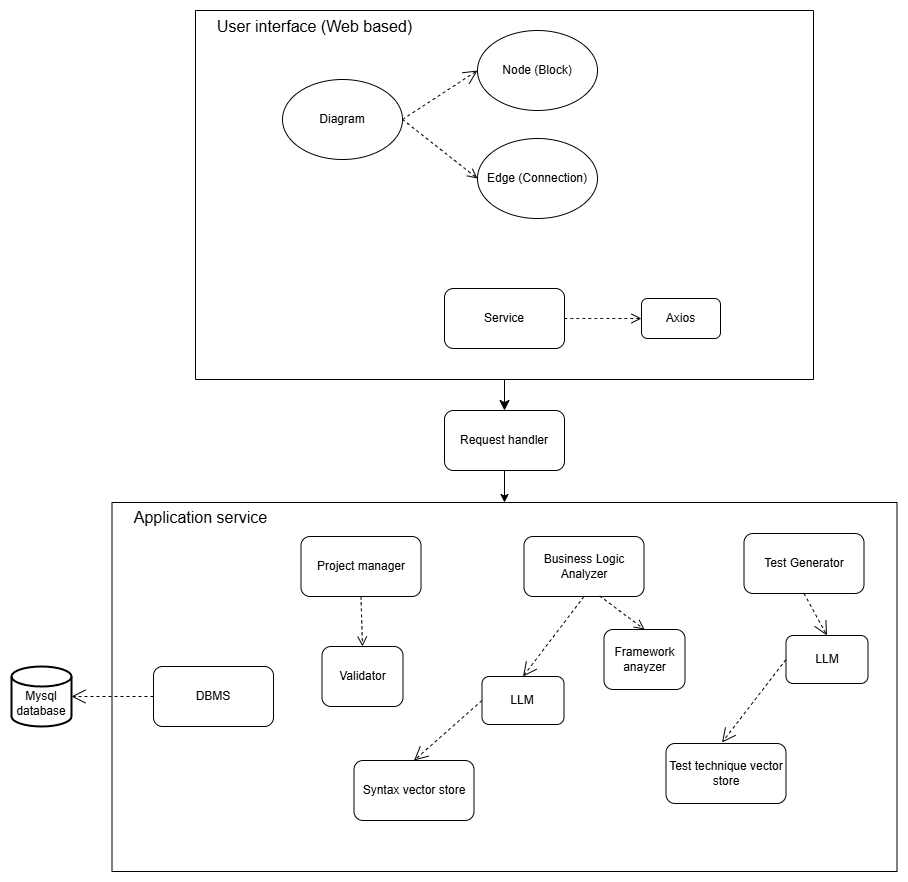
\includegraphics[width=0.8\textwidth]{images/System design.drawio.png}
	\caption{Test Genie’s overall component design}
	\label{fig:system-design}
\end{figure}

\hspace{0.5cm}\textbf{Project manager.}	This component is abstracted by framework, handle anything related to the project’s files. This component also interact with Git to clone the required project and responsible to use the SDK to validate existing tests.

\hspace{0.5cm}\textbf{BLA module}.	The BLA module plays a crucial role in analyzing the project's source code. It interacts with both project files and the database to break down the source code into components and identify relationships between classes and functions. These relationships are stored in a SQL database and visualized as component dependency diagrams to provide users with a clear representation of the project's structure. Analyzing strategy in this module will also be abstracted by framework.

\hspace{0.5cm}\textbf{Test Generator.}	This component communicates with Large Language Models (LLMs) to generate test files based on the analyzed business logic. It uses prompts and additional embedded documentation to produce runnable and framework-compliant test files that meet the project’s requirements.

\hspace{0.5cm}\textbf{Block of component ERD.}	To analyze user’s project easier, BLA module will firstly split the source files into components. These components will be connected together through different type of connection. 

\begin{figure}[H]
	\centering
	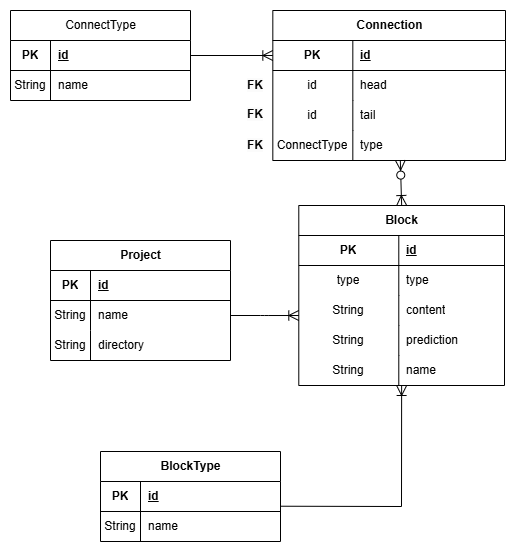
\includegraphics[width=0.8\textwidth]{images/DB block design.drawio.png}
	\caption{Block Relational Database Design}
	\label{fig:block-erd}
\end{figure}

\hspace{0.5cm}At the core of the diagram is the \textit{Block entity}, which represents distinct units of the source code identified during the project analysis. Each components stores attributes such as its type, content, prediction, and a reference to the project it belongs to. The block entity will not need to store the id of its project because it is stored as system files in the server and Backend can access it directly. This kind of design will reduce the size of the database and optimize the performance of the system.

\hspace{0.5cm} The \textit{Connection entity} defines the relationships between blocks. It uses references to two distinct blocks: head and tail, forming a directional link between them. These connections are categorized by the ConnectType entity, which stores different types of connections that can exist between blocks, such as data flow, control flow, or dependency relationships. This architecture facilitates a comprehensive understanding of the project's code structure by mapping both the functional and logical connections between different blocks.

\hspace{0.5cm}Furthermore, the \textit{BlockType entity} is used to define the classification of blocks, storing various block types such as files, classes or functions. This separation of component types allows for better categorization and analysis. The Project entity ensures that each component is tied to a specific source code directory, while ConnectType maintains clarity by classifying relationships between them. This ERD structure enables the BLA module to effectively visualize and analyze complex relationships within user projects, making it easier to identify patterns and dependencies for test generation.


% \begin{algorithm}[H]
% 	\small
% 	\caption{$(\text{Result}) \gets \texttt{Sample}(\text{Input1})$}
% 	\label{alg:1}
% 	\begin{algorithmic}[1]
% 		\Require $\text{Input1}$ is a predefined parameter.
% 		\State $\text{Set} \gets \emptyset$
% 		\For{$\text{element} \in \text{Input1}$}
% 		\If{$\text{Condition}(\text{element})$ is true}
% 		\State $\text{Set} \gets \text{Set} \cup \{\text{Process}(\text{element})\}$
% 		\Else
% 		\State \textbf{continue}
% 		\EndIf
% 		\EndFor
% 		\State $\text{Intermediate} \gets \texttt{Transform}(\text{Set})$
% 		\State \Return $\text{Result}$
% 	\end{algorithmic}
% \end{algorithm}

% Aenean arcu nulla, ornare sed arcu nec, mollis pharetra dolor. Maecenas rutrum efficitur dui nec rutrum. Sed suscipit, felis non malesuada ultrices, urna lorem porttitor mi, quis dignissim lectus mi a justo. Mauris erat ante, placerat eu sapien id, finibus maximus nisl. Nam cursus velit eu convallis molestie. Fusce eleifend fermentum elementum. Mauris congue non mauris a blandit. In vel ante mi. Etiam et consectetur quam, accumsan aliquam dolor. Aenean sed tristique massa.

\chapter{PROTOTYPING}
%% TODO: Add a small paragraph to tell what this chapter is about
This chapter delves into ...

%% TODO: Make sure to use \textbf or \textit for highlighting keywords, and \cite{} to cite the corresponding quotations

\section{System Architecture}
Fusce eros ligula, fermentum at enim at, blandit lacinia lacus. Duis malesuada mollis felis molestie aliquet. Aliquam vehicula luctus magna ac ornare. Cras eleifend metus non consequat commodo. Vivamus ultrices quam nec lacus pellentesque, ut pretium dolor interdum. Nullam cursus mauris sit amet odio laoreet cursus eget a tortor. Integer quis vulputate sem. Cras placerat fringilla tortor sit amet sagittis. Aliquam erat volutpat. Donec eleifend neque ac erat semper fringilla. Nunc ac dolor ante.

Nam congue massa ante, et hendrerit ante euismod ac. Sed fermentum diam in tempus laoreet. Pellentesque iaculis dolor eget nulla pharetra, vitae blandit tortor ullamcorper. Vestibulum vulputate tempor tellus luctus lobortis. Curabitur luctus enim vel neque rhoncus, a bibendum metus egestas. Nullam vel elementum velit. Vestibulum a lacus vel ante consequat cursus.

Duis faucibus fringilla ex ac molestie. Phasellus fringilla auctor nunc, iaculis dapibus massa dignissim sit amet. Vestibulum eget nibh faucibus, rhoncus nulla et, faucibus libero. Donec nec nisl vel quam tincidunt pretium nec id urna. Pellentesque posuere vulputate eros non rhoncus. Sed rutrum maximus orci eget pulvinar. Cras non leo eu metus suscipit gravida in at massa. Nulla faucibus, quam sed dictum elementum, mi lorem maximus quam, nec vulputate mi nisi vel ligula.

Ut varius malesuada ullamcorper. Integer ac gravida sem, sed sagittis dui. Aliquam feugiat ipsum ac maximus rutrum. Cras mollis finibus pulvinar. Quisque consectetur nisi pharetra, tempor mi vitae, vulputate urna. Pellentesque ac nulla quis sapien vehicula lacinia in vel sem. Praesent ac lorem luctus, pulvinar tellus non, condimentum velit. Nullam pulvinar condimentum ligula, quis blandit nulla laoreet porttitor. Nunc pulvinar vehicula nisi ac mattis. Nullam vestibulum quis metus a varius. Aenean ullamcorper ante nisl, a consequat diam laoreet non. Fusce faucibus malesuada lectus, non venenatis lorem lobortis ut. Donec sollicitudin laoreet nulla quis porttitor. Aenean in purus vitae erat dignissim fringilla.

\section{Strategies Choice Purposes}
Praesent id arcu odio. Mauris sed molestie lorem. Donec ipsum nisi, tincidunt non erat eu, accumsan egestas arcu. Quisque viverra rhoncus eros, vel aliquet ligula. Praesent feugiat turpis euismod risus posuere feugiat. Phasellus pharetra mi ac erat luctus semper. Suspendisse sodales purus quis risus rhoncus, at vehicula eros placerat. Nam quis mi neque.

\subsection{Strategy 1}

\subsubsection{Strategy 1 framework}
Vivamus nec venenatis ipsum, id mollis purus. Proin ultricies varius sapien, in feugiat nisl fringilla sed. Donec lobortis cursus ipsum, ut auctor velit facilisis vel. Vivamus mattis vestibulum justo nec mollis. Suspendisse potenti. Vivamus aliquet sit amet neque a vehicula. Mauris pharetra dui lorem, quis commodo sapien porta eu. In eleifend auctor justo sit amet euismod. Aliquam erat volutpat. Aliquam erat volutpat.

\chapter{IMPLEMENTATION}
%% TODO: Add a small paragraph to tell what this chapter is about
This chapter delves into the implementation of each module inside Test Genie system. Overall, this system consist of three main modules: 
\begin{itemize}
    \item[-] \textbf{Project Manager}: This module manages all the projects that are cloned to server. It mostly responsible for file-based activities and running CLI for each project.
    \item[-] \textbf{Business Logic Analyzer}: This module will take various source file from Project Manager and break the source code into smaller pieces (blocks). Then, it will analyze each block and determine what each block does and how it should be tested if possible. A test plan will also be generated for each block and save it to the database.
    \item[-] \textbf{Test Generator}: This module will take the test plan from Business Logic Analyzer and generate a test case for each block. The generated test cases will be saved as files directly in the project source code on server and can be used to run the tests later (validation).
\end{itemize}
Additionally, this system also have \textbf{DBMS} module to control the database but this module will not be explained thoroughly in this chapter.

%% TODO: Make sure to use \textbf or \textit for highlighting keywords, and \cite{} to cite the corresponding quotations

\section{Project Manager module}

The \textbf{ProjectManager} module serves as the core backend functionality for handling projects within the Test Genie system. It provides a robust framework for managing software projects by integrating Git-based repositories, file management, and testing workflows. The module is built around the \textit{Project} class, which encapsulates essential functionalities such as cloning repositories, recognizing project frameworks, and managing project files. Additionally, it features an abstract interface for test creation, validation, and execution, allowing for framework-specific extensions of functionality. For instance, the \textit{Flutter} subclass extends the \textit{Project} class to handle Flutter-specific tasks, including dependency management, `pubspec.yaml` parsing, and test execution. By modularizing these functionalities, the \textbf{ProjectManager} module streamlines project handling and enhances the system's scalability for various software development frameworks.

\subsection{Module prequisites}
This module require the SDK of supported frameworks to be installed standablone in folder \textit{./SDKs} inside the module folder. This design not only allows the module to be easily extended and modifiled to support other frameworks, but also avoid more SDK installation on the server OS. Since the \textit{Project} class (Listing A.1) just mainly control git management and file management, the subclass can freely control how the SDKs are used. \\

Subclass of Project are required to implement the following methods:
    \begin{itemize}
        \item[-] \textbf{create\_test}: This method will create the test file in the location that is required by the framework.
        \item[-] \textbf{get\_test\_content}: This method will return the content of the test file that is created by the \textbf{create\_test} method. The content of the test file is generated by the Business Logic Analyzer module.
        \item[-] \textbf{run\_test}: This method will run the test file that is created by the \textbf{create\_test} method. The test result will be returned to the caller.
        \item[-] \textbf{validate}: This method will run all the test files in the test directory and return the result. This method is used to validate the test files that are created by the \textbf{create\_test} method.
        \item[-] \textbf{getListSourceFiles}: This is an important method, which will partly decide how the source code is split into blocks. The starting point file (main file) should be placed on the first position of the list. The list will be used to split the source code into blocks. The list should contain all the source files in the project (relative to the project directory).
    \end{itemize}


\subsection{Flutter class}

The \textbf{Flutter} class extends the \textbf{Project} class to provide framework-specific support for managing Flutter projects. This class is responsible for handling operations unique to Flutter, such as managing dependencies, running tests, and validating projects. It ensures that the Flutter SDK is installed and properly configured in the \textit{./SDKs/flutter} directory before performing any operations.

Key methods of the \textbf{Flutter} class include:
\begin{itemize}
    \item[-] \textbf{\_runFlutterCLI}: This method executes commands using the Flutter CLI within the context of the project directory. It supports arguments for various Flutter commands and handles errors if the command fails.
    \item[-] \textbf{\_checkSDK}: Ensures that the Flutter SDK is installed and operational by running the \texttt{flutter --version} command. If the SDK is not present or misconfigured, the method raises an exception.
    \item[-] \textbf{\_flutterPubGet}: Automatically installs dependencies listed in the \textit{pubspec.yaml} file by running \texttt{flutter pub get}.
    \item[-] \textbf{\_addTestDependency}: Adds the Flutter \textit{test} package as a dependency using \texttt{flutter pub add test}.
    \item[-] \textbf{create\_test}: Creates a test file in the designated \textit{test} directory of the project. If the file already exists and overwriting is not allowed, an exception is raised.
    \item[-] \textbf{get\_test\_content}: Retrieves the content of a test file from the \textit{test} directory.
    \item[-] \textbf{run\_test}: Executes a specified Dart test file using the Flutter CLI and returns the results.
    \item[-] \textbf{validate}: Iterates through all Dart test files in the \textit{test} directory and validates them by running each test.
    \item[-] \textbf{getListSourceFiles}: Collects and returns a list of all source files in the \textit{lib} directory, ensuring that the \textit{main.dart} file is prioritized as the entry point.
\end{itemize}

This design enables seamless integration of Flutter-specific features into the \textbf{Test Genie} system while adhering to the modular structure defined by the \textbf{Project} class. By implementing these methods, the \textbf{Flutter} class ensures compatibility with the broader system and provides developers with a streamlined process for managing and testing Flutter projects.

\section{Business Logic Analyzer module}

\section{Test Generator module}

\section{Other implementations}
	
\chapter{RESULT}
%% TODO: Add a small paragraph to tell what this chapter is about
This chapter delves into ...

%% TODO: Make sure to use \textbf or \textit for highlighting keywords, and \cite{} to cite the corresponding quotations
\section{System Prototyping}
Integer vulputate non lectus ut sagittis. Aenean in pellentesque tellus, vel porta ex. Donec eu malesuada nibh, a eleifend velit. Class aptent taciti sociosqu ad litora torquent per conubia nostra, per inceptos himenaeos. Integer bibendum semper turpis ac bibendum. Nunc viverra justo vitae enim tincidunt gravida. Sed odio augue, scelerisque ut tincidunt eu, luctus eget ex. Duis euismod non velit et vehicula. Sed ac est porta, egestas tellus eget, convallis tortor.

\subsection{Product 1}
In sagittis nibh nec quam sodales, sit amet feugiat eros cursus. Aliquam dignissim mi vel nunc suscipit dignissim. Praesent a turpis nibh. Cras tincidunt lorem et tincidunt cursus. Cras commodo facilisis metus, quis consectetur mauris. Vestibulum eros leo, lobortis a nibh eget, congue finibus dui. Ut pharetra malesuada risus id luctus.

\section{Experiment Setup}
Integer sit amet lectus finibus, maximus sapien sit amet, efficitur turpis. Sed ut pellentesque nibh. Aliquam in quam nisl. Pellentesque ornare arcu id varius blandit. Lorem ipsum dolor sit amet, consectetur adipiscing elit. Mauris id aliquam neque. Quisque lectus sem, commodo vel libero nec, tristique rutrum elit.

\section{Experiment Result}
Duis mi felis, lobortis ut euismod vel, tristique vel ante. Curabitur in tempus dolor, eget vulputate est. Suspendisse eu facilisis ex. Nulla sodales id ipsum eu bibendum. Quisque in elementum nunc, vitae posuere augue. Ut non faucibus justo. Donec malesuada sit amet mauris sed iaculis. Vivamus tortor mauris, pretium vitae mattis pharetra, fermentum in ante. Morbi mauris dui, aliquam eu enim eget, vestibulum gravida lacus. Nullam sodales, tortor vitae fringilla efficitur, risus nisl efficitur nisl, id porta libero lacus non sem. Nulla in quam maximus, congue velit et, auctor felis. Donec tempor suscipit sollicitudin. Sed malesuada libero lectus, ut ornare purus venenatis ut.
	
\chapter{DISCUSSION}
%% TODO: Make sure to use \textbf or \textit for highlighting keywords, and \cite{} to cite the corresponding quotations
\section{Performance Analysis}

\subsection{AI generation time}

\subsection{BLA Algorithm complexity}

\subsubsection{Time Complexity}

\subsubsection{Space Complexity}

\section{Accuracy Evaluation}


\section{Comparison with Other Approach}
	
\chapter{CONCLUSION}
\section{Conclusion}
% gia tri su dung - implication

This thesis has presented Test Genie, a novel system for automated test generation in Flutter applications that addresses fundamental challenges in software testing through an innovative block-based analysis approach. By developing a solution that intelligently analyzes business logic from source code and generates human-readable, executable test cases, this research makes several significant contributions to both academic understanding and practical application in software engineering.

The central innovation of Test Genie—its block-based decomposition approach—represents a paradigm shift in how AI-driven test generation can be conceptualized. By breaking down complex codebases into semantically meaningful units, the system achieves a balance between analytical depth and computational efficiency that previous approaches have struggled to attain. This decomposition strategy effectively mitigates the source code bias problem that has plagued automated testing tools, creating tests that validate business requirements rather than merely confirming implementation details.

Empirical evaluation confirms that Test Genie achieves impressive performance characteristics, with algorithmic complexity that scales linearly with code size ($O(LOC)$) and test generation accuracy approaching 90\% after error correction. Human evaluations particularly highlighted the readability and relevance of generated tests, addressing a critical limitation of traditional automated testing approaches. These results validate the practical utility of the system in real-world development scenarios, where it demonstrated a 62\% reduction in time spent writing tests compared to manual authoring.

Beyond its immediate practical applications, this research carries broader implications for software engineering practices. The human-in-the-loop design philosophy embedded throughout Test Genie demonstrates how AI and human expertise can be synergistically combined, leveraging the strengths of each while mitigating their respective weaknesses. This collaborative approach represents a promising direction for AI-augmented software engineering tools that enhance developer productivity without diminishing human agency or understanding.

In addressing the challenge of automated test generation for the Flutter framework, this thesis makes a meaningful contribution to the growing field of mobile and cross-platform application development. As these frameworks continue to evolve and gain popularity, the need for efficient testing methodologies becomes increasingly acute. Test Genie establishes a foundation upon which more sophisticated testing approaches can be built, potentially influencing the design of both testing tools and frameworks themselves.

From an academic perspective, this research advances understanding of how large language models can be effectively applied to specialized software engineering tasks. The retrieval-augmented generation approach employed in Test Genie demonstrates how domain-specific knowledge can be incorporated into AI systems to improve accuracy and relevance in technical contexts. This contributes to the broader discourse on adapting general-purpose AI technologies to specialized domains.

The interdisciplinary nature of this work—bridging software engineering, artificial intelligence, and human-computer interaction—highlights the increasingly blurred boundaries between these fields. As software systems grow more complex and AI capabilities more sophisticated, such interdisciplinary approaches become not merely beneficial but essential. Test Genie exemplifies how insights from multiple disciplines can be integrated to create tools that address complex challenges in ways that single-discipline approaches cannot.

In conclusion, Test Genie represents a significant advancement in automated test generation, offering both immediate practical value through enhanced testing efficiency and broader implications for how AI can be thoughtfully integrated into software development workflows. By balancing technical sophistication with usability, and automation with human oversight, this system establishes a model for AI-augmented development tools that enhance rather than replace human capabilities. As software continues to pervade every aspect of modern life, such tools will play an increasingly vital role in ensuring software quality, reliability, and security.

\section{Future Work}

While Test Genie has demonstrated significant advances in automated test generation for Flutter applications, several promising research directions remain to be explored. These potential extensions would address current limitations and further enhance the system's capabilities.

First, expanding framework support beyond Flutter represents a natural evolution of this research. The block-based decomposition approach developed in this thesis could be adapted to other mobile and web frameworks such as React Native, Angular, or SwiftUI. This expansion would require developing framework-specific analyzers and test generators, but the core architectural concepts should transfer effectively. Comparative studies across different frameworks might also yield insights into architectural patterns that are particularly amenable to automated testing.

Second, enhancing the system's handling of complex state management represents a critical area for improvement. As noted in the evaluation, Test Genie's performance decreased when dealing with sophisticated state management patterns like BLoC or Redux. Future research could explore specialized analysis techniques for these patterns, potentially incorporating static flow analysis to better understand state transformations and dependencies. This would address one of the most challenging aspects of modern application testing.

Third, the current test validation approach focuses primarily on syntactic correctness and runnability. A valuable extension would be developing techniques to evaluate test quality and coverage more comprehensively. This might include measuring assertion quality, behavior coverage (rather than just code coverage), and alignment with business requirements. Such advancements would help ensure that generated tests provide meaningful validation rather than superficial verification.

Fourth, investigating the potential for reinforcement learning with human feedback (RLHF) could significantly improve prediction accuracy. By systematically collecting and incorporating user corrections of block predictions, the system could continuously refine its understanding of business logic patterns. This approach would leverage the human-in-the-loop architecture already present in Test Genie while reducing the need for manual intervention over time.

Fifth, as mobile applications increasingly leverage platform-specific features, improving the generation of tests for platform channels and native code integration represents an important challenge. Future work could explore techniques for analyzing cross-language interfaces and generating appropriate mocks and test harnesses for platform-specific components.

Finally, integrating Test Genie with continuous integration and deployment pipelines would enhance its practical utility in professional development environments. Research into effective integration patterns, incremental test updating based on code changes, and optimization for performance in CI environments would make the system more applicable to real-world development workflows.

These research directions would build upon the foundation established in this thesis, addressing existing limitations while extending the applicability and effectiveness of AI-driven test generation systems. As software continues to grow in complexity and criticality, such advancements will become increasingly valuable for ensuring quality, reliability, and security.

\bibliographystyle{ieeetr}
\bibliography{bibliography.bib}

\begin{thebibliography}{9}
\bibitem{WQR2122}
Capgemini - “World Quality Report 2021-22”, Thirdteenth edition.

\bibitem{QASalaries}
Glassdoor - “Qa Tester Salaries”, https://www.glassdoor.com/Salaries/qa-tester-salary-SRCH\_KO0,9.htm 

\bibitem{CostPoorSoftware}
Herb Krasner, Consortium for information \& Software quality - ``The Cost of Poor Software Quality in the US: A 2020 Report''.

\bibitem{flask}
Migual Gringerg - “Flask Web Development”, 2014, Published by O'Reilly Media, Inc.

\bibitem{langchain}
“Langchain”, https://python.langchain.com/docs/introduction/ 

\bibitem{PyMachineLearning}
Abhishek Singh - “Essential Python for Machine Learning”, new edition 2023.

\bibitem{UnitTest}
Shreya Bhatia, Tarushi Gandhi, Dhruv Kumar, Pankaj Jalote - “Unit Test Generation using Generative AI : A Comparative Performance Analysis of Autogeneration Tools”

\bibitem{LLMLimitations}
Tosin Adewumi, Nudrat Habib, Lama Alkhaled \& Elisa Barney ML Group, EISLAB, Luleå University of Technology, Sweden - “On the Limitations of Large Language Models (LLMs): False Attribution”.


\bibitem{BusinessRules}
Harry M. Sneed, Katalin Erdos - “Extracting Business Rules from Source Code”, April 1996

\bibitem{codeMeasures}
Adrian S. Barb, Colin J. Neill, Raghvinder S. Sangwan, Michael J. Piovoso – “A statistical study of the relevance of lines of code measures in software projects”, May 7, 2014.

\end{thebibliography}

\appendix
\chapter{LISTINGS}
\begin{lstlisting}[language=JavaScript, caption={$\texttt{Sample}$ procedure.}, label={lst:1}]
    function calculateSumAndProduct(input) {
      const pattern = /^X(\d{2})Y(\d{2})$/;
      const match = input.match(pattern);
    
      if (!match) {
        throw new Error("Invalid format! Expected format: X[XX]Y[YY]");
      }
    
      const firstNumber = parseInt(match[1], 10);
      const secondNumber = parseInt(match[2], 10);
    
      const sum = firstNumber + secondNumber;
      const product = firstNumber * secondNumber;
    
      console.log(`Input: ${input}`);
      console.log(`Sum: ${firstNumber} + ${secondNumber} = ${sum}`);
    }
    
    // Example usage
    try {
      calculateSumAndProduct("X12Y34"); // Valid case
      calculateSumAndProduct("X05Y07"); // Valid case
      calculateSumAndProduct("A12B34"); // Invalid case
    } catch (error) {
      console.error(error.message);
    }
    \end{lstlisting}

\end{document}